\documentclass[class=article,crop=false]{standalone} \usepackage[margin=1in,headheight=57pt,headsep=0.1in]{geometry}
\usepackage[subpreambles=true]{standalone}
\usepackage{float}
\usepackage[framemethod=TikZ]{mdframed}
\usepackage{fancyhdr}
\usepackage[utf8]{inputenc} % Required for inputting international characters
\usepackage[T1]{fontenc} % Output font encoding for international characters
\usepackage{stix} % Use the STIX fonts
\usepackage{hyperref}
\hbadness=99999

\begin{document}
\subsection{The Introduction Form}
\begin{figure}[H]
	\centering
	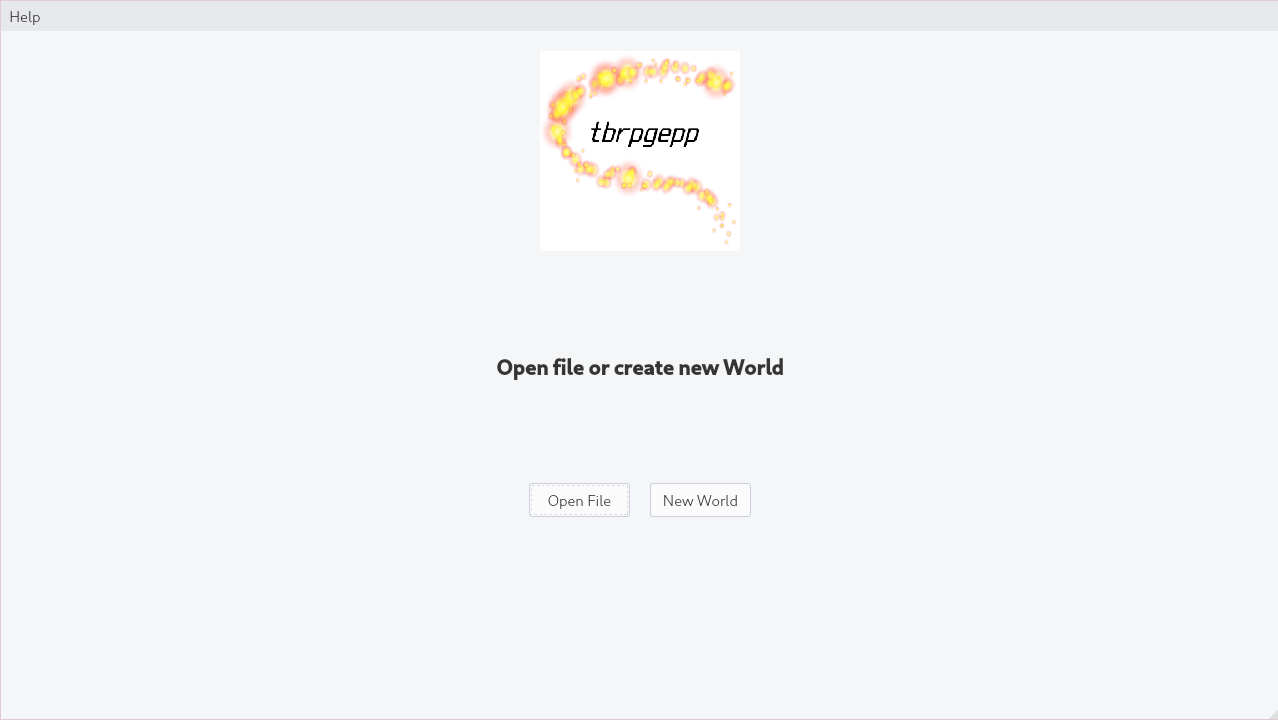
\includegraphics[width=1.0\textwidth]{./introForm.png}
\end{figure}
This is the first form you see when you execute the \texttt{mainMenuForm.py} file. You are presented with two options: open a preexisting file containing a \texttt{tbrpggepp} game world, or create a new one.
\subsubsection{Creating a new game-world}
\begin{figure}[H]
	\centering
	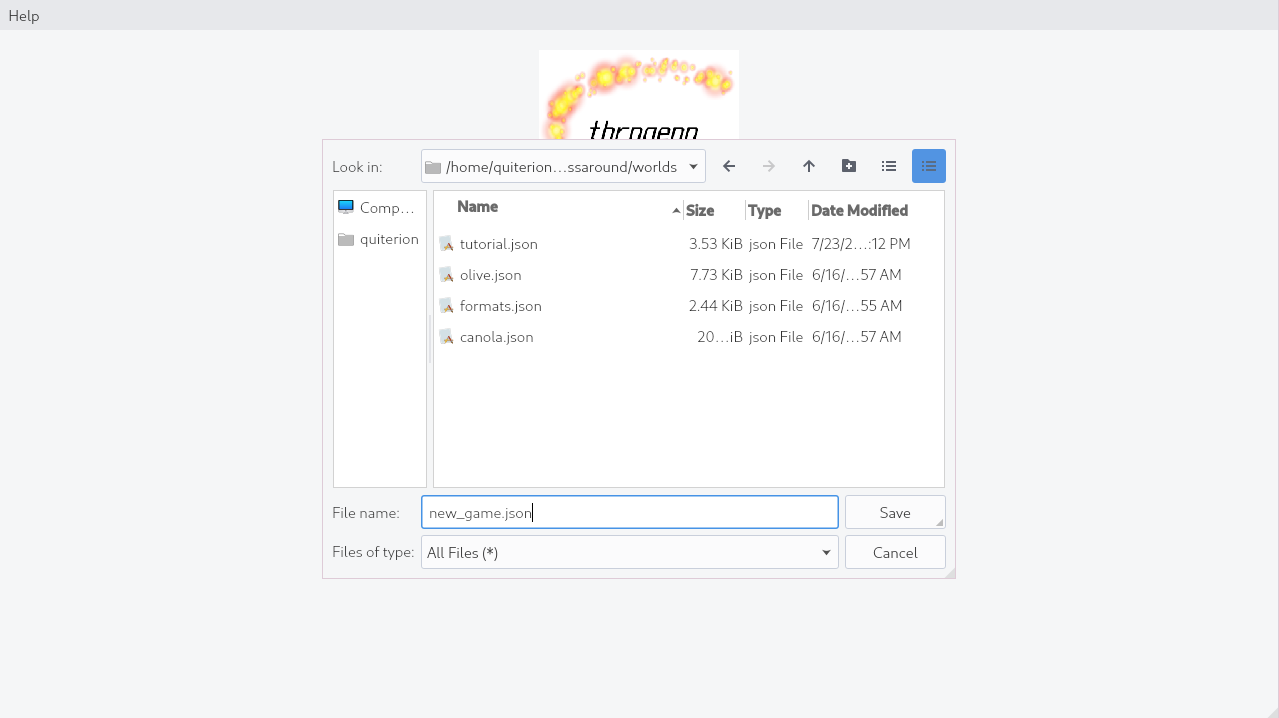
\includegraphics[width=1.0\textwidth]{./introFormWithFileDialog.png}
\end{figure}
Upon clicking "New World", a dialog will appear prompting you to create a new file. You may create this file in any directory you please, but \textbf{note that game-world files must have a "\texttt{.json}" extension.} After creating a file, the Introduction form will close and take you to the Main Menu form.
\subsubsection{Opening a preexisting game-world file}
\begin{figure}[H]
	\centering
	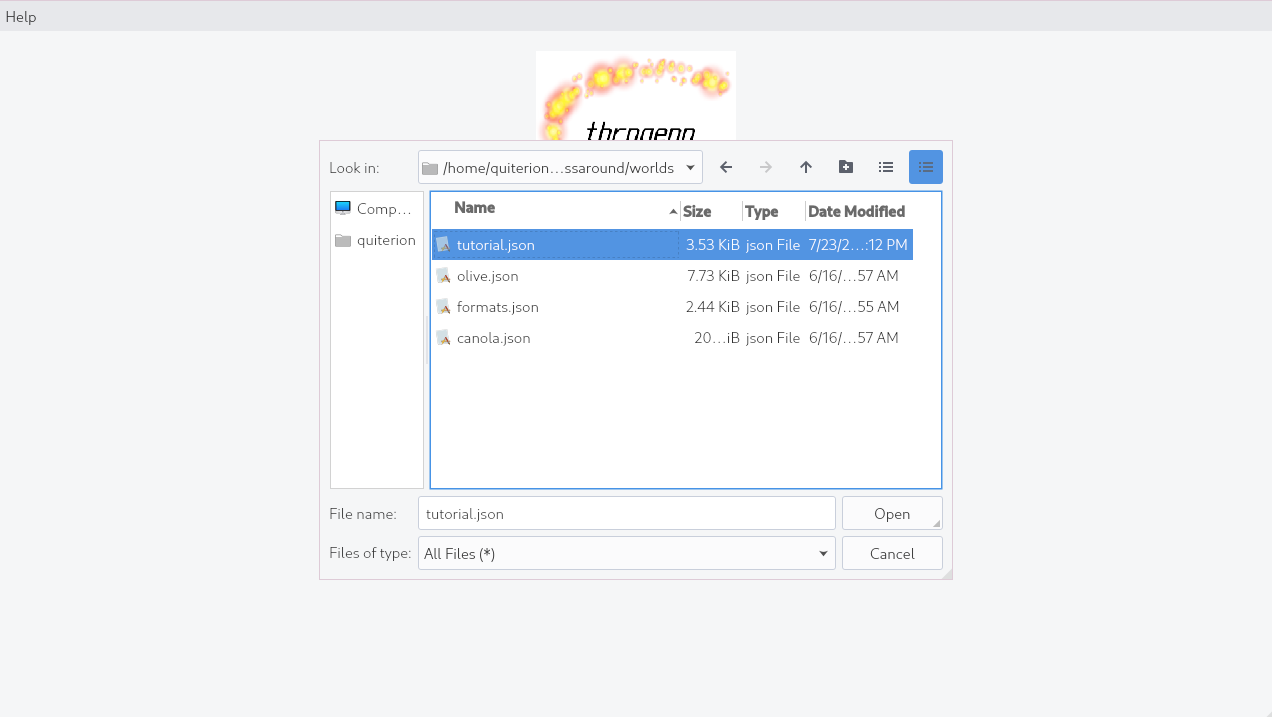
\includegraphics[width=1.0\textwidth]{./introFormWithOpenFileDialog.png}
\end{figure}
Upon clicking "Open File" an identical dialog will appear, this time prompting you to select a preexisting file. \textbf{Note that a valid game-world file must end in a "\texttt{.json}" extension.} After selecting a file, the Introduction form will close and take you to the Main Menu form.
\end{document}
